% % % % % % % % % % % % % % % % % % % % % % % % % % % % % % % % % % % % % % % %
% IEEE Style - Double columns, 11pt font, letterpaper
\documentclass[journal, twocolumn, final,11pt,letterpaper]{IEEEtran}	

% Include Latex Packages
\usepackage{etex}	% This package enables the use of many packages

% % Page styles
\usepackage{setspace}	% line spacing package
\doublespacing			% use double spacing
%\linespread{1.6}		% Use linespread to fine tune line spacing, not recommended


% % Figures
\usepackage{float}		% improves interface for floating objects
\usepackage{subfig}		% enables subfloat
\usepackage{graphicx}	% more image type support
\usepackage{circuitikz}
\usepackage{epstopdf}	% automatically convert included eps files to pdf
\usepackage{tikz}
%\usepackage{listings}
\usepackage{color}
\definecolor{dkgreen}{rgb}{0,0.6,0}
\definecolor{gray}{rgb}{0.5,0.5,0.5}
\definecolor{mauve}{rgb}{0.58,0,0.82}

\lstset{frame=tb,
	language=Verilog,
	aboveskip=3mm,
	belowskip=3mm,
	showstringspaces=false,
	columns=flexible,
	basicstyle={\small\ttfamily},
	numbers=none,
	numberstyle=\tiny\color{gray},
	keywordstyle=\color{blue},
	commentstyle=\color{dkgreen},
	stringstyle=\color{mauve},
	breaklines=true,
	breakatwhitespace=true,
	tabsize=3
}
\usetikzlibrary{matrix,calc}
\usetikzlibrary{shapes}

\newcommand*{\circled}[2][red]{
	\tikz[baseline=(char.base)]{
		\node[shape=ellipse,inner sep=1pt,
		draw=#1,
		] (char) {#2};}
}

%isolated term
%#1 - Optional. Space between node and grouping line. Default=0
%#2 - node
%#3 - filling color
\newcommand{\implicantsol}[3][0]{
	\draw[rounded corners=3pt, fill=#3, opacity=0.3] ($(#2.north west)+(135:#1)$) rectangle ($(#2.south east)+(-45:#1)$);
}


%internal group
%#1 - Optional. Space between node and grouping line. Default=0
%#2 - top left node
%#3 - bottom right node
%#4 - filling color
\newcommand{\implicant}[4][0]{
	\draw[rounded corners=3pt, fill=#4, opacity=0.3] ($(#2.north west)+(135:#1)$) rectangle ($(#3.south east)+(-45:#1)$);
}

%group lateral borders
%#1 - Optional. Space between node and grouping line. Default=0
%#2 - top left node
%#3 - bottom right node
%#4 - filling color
\newcommand{\implicantcostats}[4][0]{
	\draw[rounded corners=3pt, fill=#4, opacity=0.3] ($(rf.east |- #2.north)+(90:#1)$)-| ($(#2.east)+(0:#1)$) |- ($(rf.east |- #3.south)+(-90:#1)$);
	\draw[rounded corners=3pt, fill=#4, opacity=0.3] ($(cf.west |- #2.north)+(90:#1)$) -| ($(#3.west)+(180:#1)$) |- ($(cf.west |- #3.south)+(-90:#1)$);
}

%group top-bottom borders
%#1 - Optional. Space between node and grouping line. Default=0
%#2 - top left node
%#3 - bottom right node
%#4 - filling color
\newcommand{\implicantdaltbaix}[4][0]{
	\draw[rounded corners=3pt, fill=#4, opacity=0.3] ($(cf.south -| #2.west)+(180:#1)$) |- ($(#2.south)+(-90:#1)$) -| ($(cf.south -| #3.east)+(0:#1)$);
	\draw[rounded corners=3pt, fill=#4, opacity=0.3] ($(rf.north -| #2.west)+(180:#1)$) |- ($(#3.north)+(90:#1)$) -| ($(rf.north -| #3.east)+(0:#1)$);
}

%group corners
%#1 - Optional. Space between node and grouping line. Default=0
%#2 - filling color
\newcommand{\implicantcantons}[2][0]{
	\draw[rounded corners=3pt, opacity=.3] ($(rf.east |- 0.south)+(-90:#1)$) -| ($(0.east |- cf.south)+(0:#1)$);
	\draw[rounded corners=3pt, opacity=.3] ($(rf.east |- 8.north)+(90:#1)$) -| ($(8.east |- rf.north)+(0:#1)$);
	\draw[rounded corners=3pt, opacity=.3] ($(cf.west |- 2.south)+(-90:#1)$) -| ($(2.west |- cf.south)+(180:#1)$);
	\draw[rounded corners=3pt, opacity=.3] ($(cf.west |- 10.north)+(90:#1)$) -| ($(10.west |- rf.north)+(180:#1)$);
	\fill[rounded corners=3pt, fill=#2, opacity=.3] ($(rf.east |- 0.south)+(-90:#1)$) -|  ($(0.east |- cf.south)+(0:#1)$) [sharp corners] ($(rf.east |- 0.south)+(-90:#1)$) |-  ($(0.east |- cf.south)+(0:#1)$) ;
	\fill[rounded corners=3pt, fill=#2, opacity=.3] ($(rf.east |- 8.north)+(90:#1)$) -| ($(8.east |- rf.north)+(0:#1)$) [sharp corners] ($(rf.east |- 8.north)+(90:#1)$) |- ($(8.east |- rf.north)+(0:#1)$) ;
	\fill[rounded corners=3pt, fill=#2, opacity=.3] ($(cf.west |- 2.south)+(-90:#1)$) -| ($(2.west |- cf.south)+(180:#1)$) [sharp corners]($(cf.west |- 2.south)+(-90:#1)$) |- ($(2.west |- cf.south)+(180:#1)$) ;
	\fill[rounded corners=3pt, fill=#2, opacity=.3] ($(cf.west |- 10.north)+(90:#1)$) -| ($(10.west |- rf.north)+(180:#1)$) [sharp corners] ($(cf.west |- 10.north)+(90:#1)$) |- ($(10.west |- rf.north)+(180:#1)$) ;
}

%Empty Karnaugh map 4x4
\newenvironment{Karnaugh}%
{
	\begin{tikzpicture}[baseline=(current bounding box.north),scale=0.8]
	\draw (0,0) grid (4,4);
	\draw (0,4) -- node [pos=0.9,above right,anchor=south west] {C1C0} node [pos=0.9,below left,anchor=north east] {EQ} ++(135:1);
	%
	\matrix (mapa) [matrix of nodes,
	column sep={0.8cm,between origins},
	row sep={0.8cm,between origins},
	every node/.style={minimum size=0.3mm},
	anchor=8.center,
	ampersand replacement=\&] at (0.5,0.5)
	{
		\& |(c00)| 00         \& |(c01)| 01         \& |(c11)| 11         \& |(c10)| 10         \& |(cf)| \phantom{00} \\
		|(r00)| 00             \& |(0)|  \phantom{0} \& |(1)|  \phantom{0} \& |(3)|  \phantom{0} \& |(2)|  \phantom{0} \&                     \\
		|(r01)| 01             \& |(4)|  \phantom{0} \& |(5)|  \phantom{0} \& |(7)|  \phantom{0} \& |(6)|  \phantom{0} \&                     \\
		|(r11)| 11             \& |(12)| \phantom{0} \& |(13)| \phantom{0} \& |(15)| \phantom{0} \& |(14)| \phantom{0} \&                     \\
		|(r10)| 10             \& |(8)|  \phantom{0} \& |(9)|  \phantom{0} \& |(11)| \phantom{0} \& |(10)| \phantom{0} \&                     \\
		|(rf) | \phantom{00}   \&                    \&                    \&                    \&                    \&                     \\
	};
}%
{
	\end{tikzpicture}
}

%Empty Karnaugh map 2x4
\newenvironment{Karnaughvuit}%
{
	\begin{tikzpicture}[baseline=(current bounding box.north),scale=0.8]
	\draw (0,0) grid (4,2);
	\draw (0,2) -- node [pos=0.7,above right,anchor=south west] {LA/LB} node [pos=0.6,below left,anchor=north east] {S} ++(120:1);
	%
	\matrix (mapa) [matrix of nodes,
	column sep={0.8cm,between origins},
	row sep={0.8cm,between origins},
	every node/.style={minimum size=0.3mm},
	anchor=4.center,
	ampersand replacement=\&] at (0.5,0.5)
	{
		\& |(c00)| 00         \& |(c01)| 01         \& |(c11)| 11         \& |(c10)| 10         \& |(cf)| \phantom{00} \\
		|(r00)| 0             \& |(0)|  \phantom{0} \& |(1)|  \phantom{0} \& |(3)|  \phantom{0} \& |(2)|  \phantom{0} \&                     \\
		|(r01)| 1             \& |(4)|  \phantom{0} \& |(5)|  \phantom{0} \& |(7)|  \phantom{0} \& |(6)|  \phantom{0} \&                     \\
		|(rf) | \phantom{00}  \&                    \&                    \&                    \&                    \&                     \\
	};
}%
{
	\end{tikzpicture}
}

%Empty Karnaugh map 2x2
\newenvironment{Karnaughquatre}%
{
	\begin{tikzpicture}[baseline=(current bounding box.north),scale=0.8]
	\draw (0,0) grid (2,2);
	\draw (0,2) -- node [pos=0.7,above right,anchor=south west] {b} node [pos=0.7,below left,anchor=north east] {a} ++(135:1);
	%
	\matrix (mapa) [matrix of nodes,
	column sep={0.8cm,between origins},
	row sep={0.8cm,between origins},
	every node/.style={minimum size=0.3mm},
	anchor=2.center,
	ampersand replacement=\&] at (0.5,0.5)
	{
		\& |(c00)| 0          \& |(c01)| 1  \\
		|(r00)| 0 \& |(0)|  \phantom{0} \& |(1)|  \phantom{0} \\
		|(r01)| 1 \& |(2)|  \phantom{0} \& |(3)|  \phantom{0} \\
	};
}%
{
	\end{tikzpicture}
}

%Defines 8 or 16 values (0,1,X)
\newcommand{\contingut}[1]{%
	\foreach \x [count=\xi from 0]  in {#1}
	\path (\xi) node {\x};
}

%Places 1 in listed positions
\newcommand{\minterms}[1]{%
	\foreach \x in {#1}
	\path (\x) node {1};
}

%Places 0 in listed positions
\newcommand{\maxterms}[1]{%
	\foreach \x in {#1}
	\path (\x) node {0};
}

%Places X in listed positions
\newcommand{\indeterminats}[1]{%
	\foreach \x in {#1}
	\path (\x) node {X};
}



% % Maths
\usepackage[cmex10]{amsmath}	% Maths
\usepackage{amsfonts,amssymb} 	% maths symbols

% % Tables
\usepackage{booktabs}  % professional-looking tables
\usepackage{multicol} %used for getting multicolumn without page-break
\usepackage{multirow}	% multi-row tables
\usepackage{array}		% define column format of a table

% % Others
\usepackage{caption}	%Customising captions in floating environments
%\usepackage{abstract}
\usepackage{cite}		% cite multiple
\usepackage{fixltx2e}	%added by pilawa, preventing figure* to get ahead of regular figures.
\usepackage{url}		% url display

% %
\hyphenation{op-tical net-works semi-conduc-tor}	% correct bad hyphenation here
\providecommand{\e}[1]{\ensuremath{\times 10^{#1}}}		% use use \e{2} for scientific number expression


% % Optional packages that might be useful
%\usepackage{epsf}		% eps fix
%\usepackage{verbatim}	% verbatim text are not interpreted by the compiler 
%\numberwithin{equation}{section}	% number equation according to section
%\usepackage{xfrac}		% slanted fraction
%\usepackage{pgfplots}	% plot graph
%\usepackage{tikz,pgfplots} % plot graph
%\usepackage{endnotes}	% endnotes


% Title of Document
\title{ECE385 Experiment \#8
	}
\author{
\IEEEauthorblockN{Eric Meyers, Ryan Helsdingen}\\
\IEEEauthorblockA{Section ABG; TAs: Ben Delay, Shuo Liu \\
March 30th, 2016 \\
emeyer7, helsdin2}}
% % % % % % % % % % % % % % % % % % % % % % % % % % % % % % % % % % % % % % % 
\begin{document}
	
%SECTION : Formatting and Title
\maketitle
\singlespacing

%SECTION 1 - Introduction - Eric
\section{Introduction}
The purpose of this lab is to introduce concepts pertaining to USB protocol/communication and VGA display. The main goal of this lab was to connect a USB keyboard to the Altera FPGA and allow a user to control a ball displayed on a VGA-connected monitor.

%SECTION 2 - Description of Circuit / Inputs and Outputs - 
\section{Description of Circuit}
RYAN SECTION

%SECTION 3 - Purpose of Modules - 
\section{Purpose of Modules}
RYAN SECTION

%SECTION 4 - Description of USB Protocol & Changes
\section{Description of USB Protocol \& Changes}
The USB protocol in Experiment 8 utilized the Cypress EZ-OTG (CY7C67200) USB controller on board the Altera. The CY7C67200 was used as a host controller and once a USB keyboard is plugged in, the keyboard acts as a device controller.\\

The USB Keyboard is not an interrupt-based device, rather the host must poll the keyboard and send requests to receive the scancode in return. For this, the team must write functions to perform input/output reading and writing. These functions must be used in conjunction with the system verilog hardware that is synthesized to retrieve data and write data. 

The two functions that were written by the team were in "usb.c" and "io\_handler.c" were pertaining to the reading and writing of data to and from the USB device controller (keyboard).\\

io\_handler.c:
\begin{itemize}
	\item 	void IO\_init(void)
	\item 	void IO\_write(alt\_u8 Address, alt\_u16 Data)
\end{itemize}


\begin{lstlisting}
void IO_write(alt_u8 Address, alt_u16 Data)
{
	*otg_hpi_address = Address;
	*otg_hpi_cs = 0;
	*otg_hpi_w = 0;
	*otg_hpi_data = Data;
	*otg_hpi_w = 1;
	*otg_hpi_cs = 1;
}
\end{lstlisting}
This function takes in parameters as the Address and Data to be written. It then sets the appropriate bits on the signal lines and sends the Data to the otg\_hpi\_data variable to be written to the usb hardware.\\ 

\begin{lstlisting}
alt_u16 IO_read(alt_u8 Address)
{
	alt_u16 temp;
	//printf("%x\n",temp);
	*otg_hpi_address = Address;
	*otg_hpi_cs = 0;
	*otg_hpi_r = 0;
	temp = *otg_hpi_data;
	*otg_hpi_r = 1;
	*otg_hpi_cs = 1;
	return temp;
}
\end{lstlisting}
This function performs similar actions to the IO\_write function in that it must read from a particular address on the USB hardware. The team had to use a temp variable to read it properly, set the appropriate signals, then send the data from otg\_hpi\_data into the temp variable which is then returned to the user by the function.\\

usb.c:
\begin{itemize}
	\item 	void UsbWrite(alt\_u16 Address, alt\_u16 Data)
	\item 	alt\_u16 UsbRead(alt\_u16 Address)
\end{itemize}
\begin{lstlisting}
void UsbWrite(alt_u16 Address, alt_u16 Data)
{
	IO_write(HPI_ADDR, Address);
	IO_write(HPI_DATA, Data);
}
\end{lstlisting}
This function utilizes the two functions written in the previous section (in io\_handler.c) and simply writes the particular address and the data in the parameters.


\begin{lstlisting}
alt_u16 UsbRead(alt_u16 Address)
{
	IO_write(HPI_ADDR, Address);
	alt_u16 temp = IO_read(HPI_DATA);
	return temp;
}
\end{lstlisting}
This function uses the two functions written in io\_handler.c to perform a read on the USB hardware. it first must write the address to HPI\_ADDR to receive the proper address, then the temp variable must store the result of IO\_read from HPI\_Data. 



%SECTION 5 - Schematic/Block Diagram - 
\section{Schematic/Block Diagram}
The Schematic / Block Diagrams for this lab can be found in the Figures section of this document ("Section XI: Figures"). The Top Level Module Diagram can be found in Figure \ref{fig:top-level}, the Ball Module Diagram can be found in Figure \ref{fig:ball}, the VGA Module Diagram can be found in Figure \ref{fig:vga}, and the Color Mapper Module can be found in Figure \ref{fig:color_mapper}.

%SECTION 6 - Post Lab - 
\section{Post Lab}
\begin{table}[htbp]
	\centering
	\begin{tabular}{c|c}	% ccccccc indicates 7 center aligned columns
		\toprule	% top separator
		Resource & Value \\
		\midrule
		LUT & 2663\\
		DSP & 10\\
		Memory (BRAM) & 82,944\\
		Flip-Flop & 646\\
		Frequency &   132.89 MHz\\
		Static Power & 102.09 mW\\
		Dynamic Power &  25.86 mW\\
		Total Power & 203.64 mW\\
		\bottomrule	% bottom separator
	\end{tabular}%	
	\caption{Design Statistics}
	\label{tab:design}
\end{table}

1. What is the difference between VGA\_clk and Clk? \\

\textit{Answer:}The VGA Clock runs at 25MHz to change how wide the individual pixels are, whereas the Clk onboard the processor runs at 50MHz (and does not affect the pixel size).\\

2. In the file io\_handler.h, why is it that the otg\_hpi\_address is defined as an integer pointer while the otg\_hpi\_r is defined as a char pointer? \\

\textit{Answer:} otg\_hpi\_r is a single bit and does not need to be declared as an int (16 bits - it would be a waste of space), whereas otg\_hpi\_address is multiple bits wide and must have multiple bits available to use.\\

3.What are the advantages and/or disadvantages of using a USB interface over PS/2 interface to connect to the keyboard? List any two. \\

\textit{Answer:} PS/2 keyboards aren't polled, but are completely interrupt based. This allows the processor to complete tasks while waiting. Drivers for PS/2 are much simpler than USB keyboard drivers. Another disadvantage is that the USB keyboard only takes in 6 keys every message, so this is limited compared to the PS/2. These are two disadvantages for using a USB keyboard over PS/2.\\

4.  Note that Ball\_Y\_Motion in the above statement may have been changed at the same clock edge that is causing the assignment of Ball\_Y\_pos.  Will the new value of Ball\_Y\_Motion be used, or the old?  How will this impact behavior of the ball during a bounce, and how might that interact with a response to a keypress?  Can you fix it?\\

\textit{Answer:} The new value of Ball\_Y\_Motion that would be used would be the old one and this would make it so that the ball bounces one clock cycle after the keypress is handled. A fix would be to put the assignment inside of the section of code that bounces the ball so that there is no delay in processing. \\

%SECTION 7 - Conclusion
\section{Conclusion}
RYAN SECTION

\clearpage
\onecolumn
%SECTION 11: Figures
\section{Figures}

\begin{figure} [H]
	\centering
	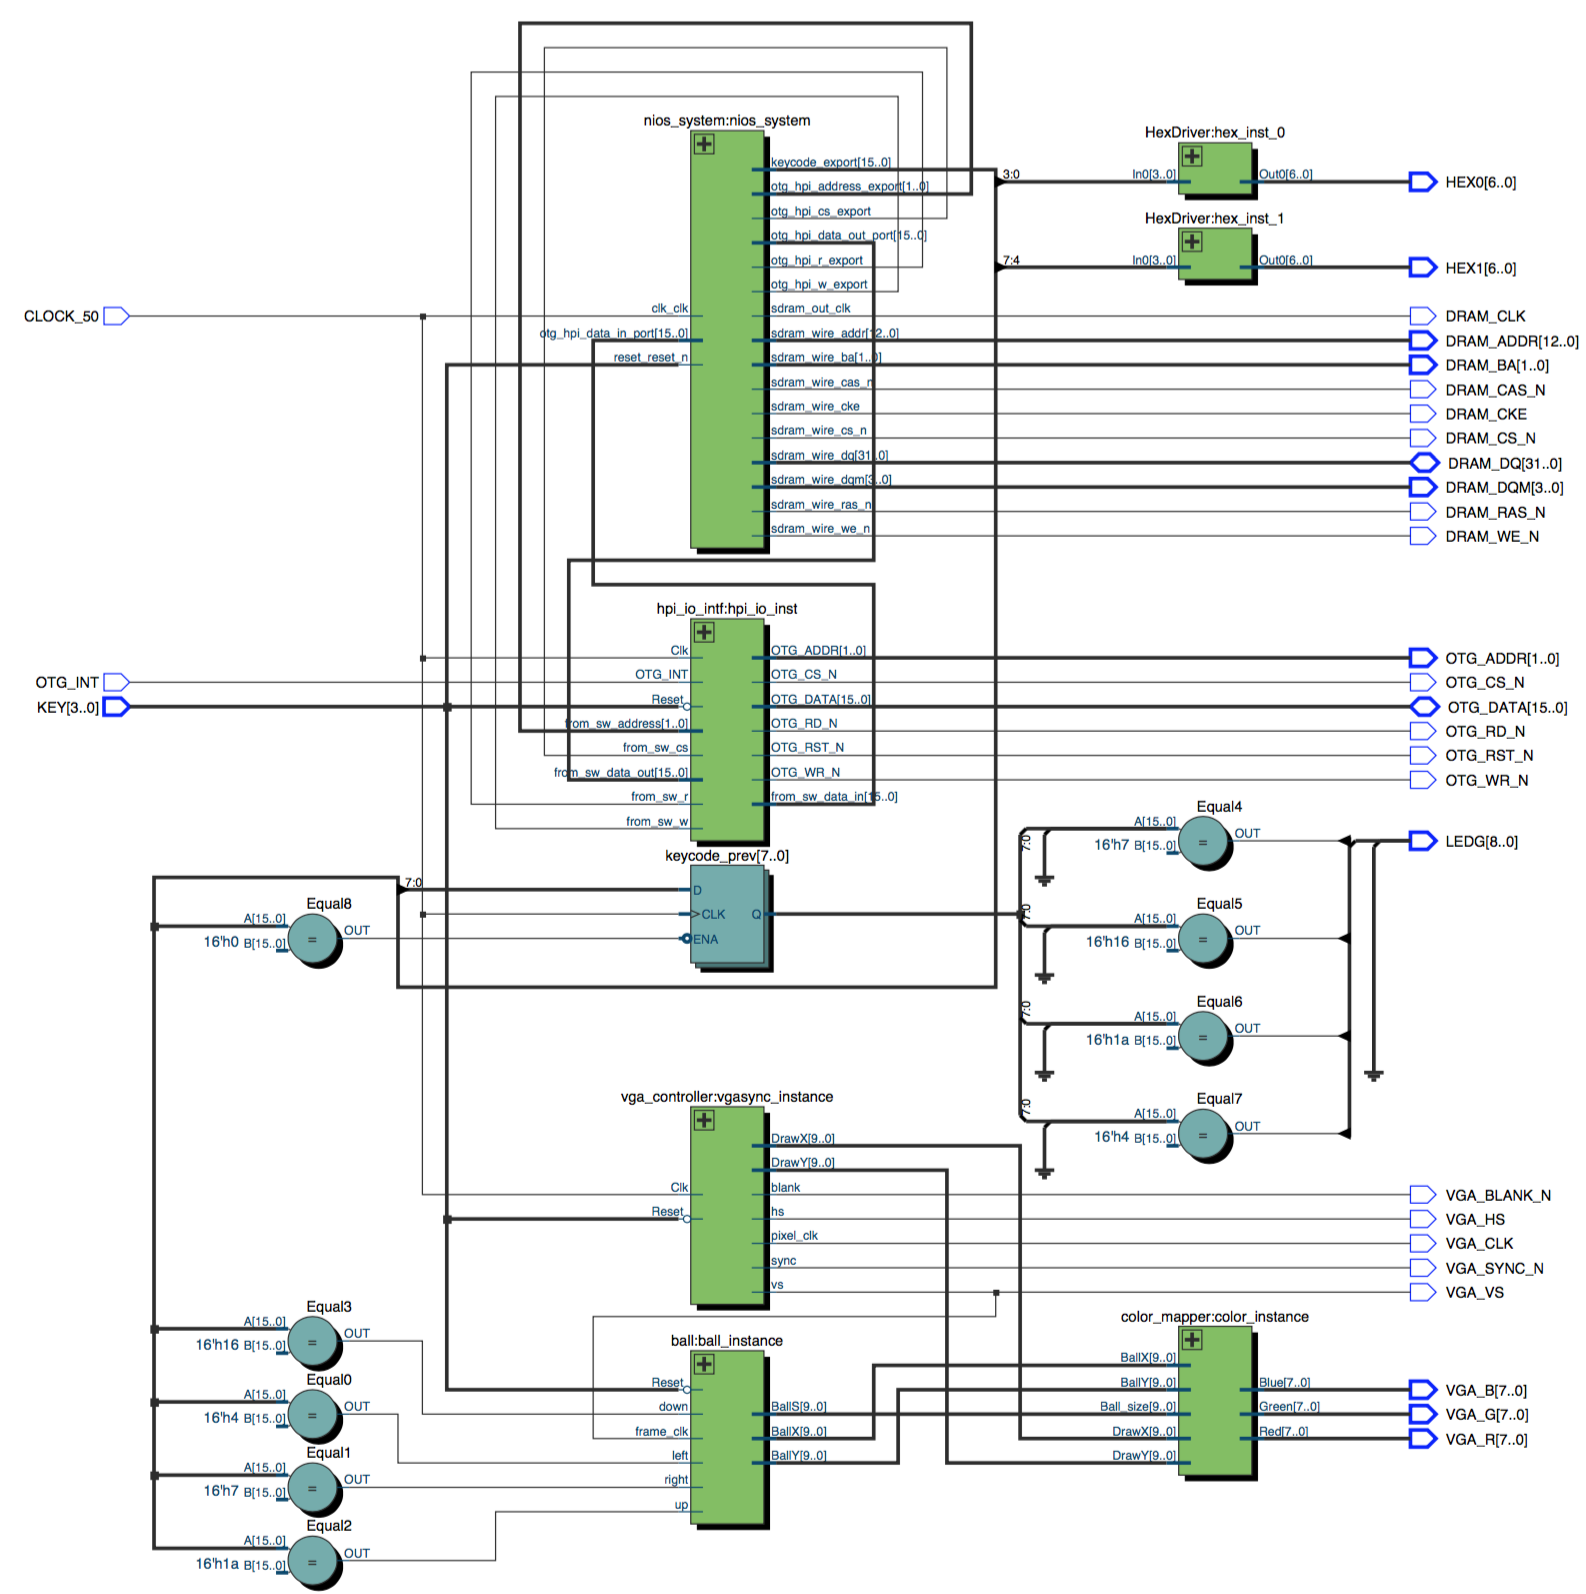
\includegraphics[scale=.5]{top_level_diagram.png}
	\caption{Lab 8 Top Level SV\label{fig:top-level}}
\end{figure}

\begin{figure} [H]
	\centering
	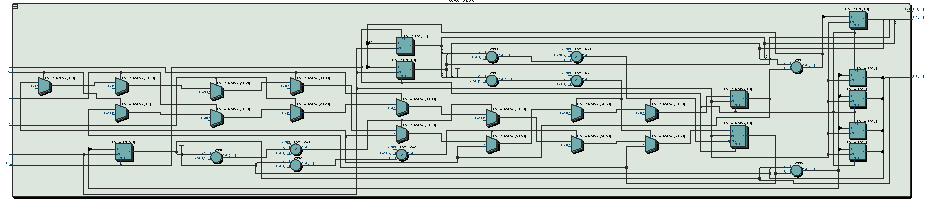
\includegraphics[scale=1]{ball_diagram.pdf}
	\caption{Ball Circuit Diagram\label{fig:ball}}
\end{figure}

\begin{figure} [H]
	\centering
	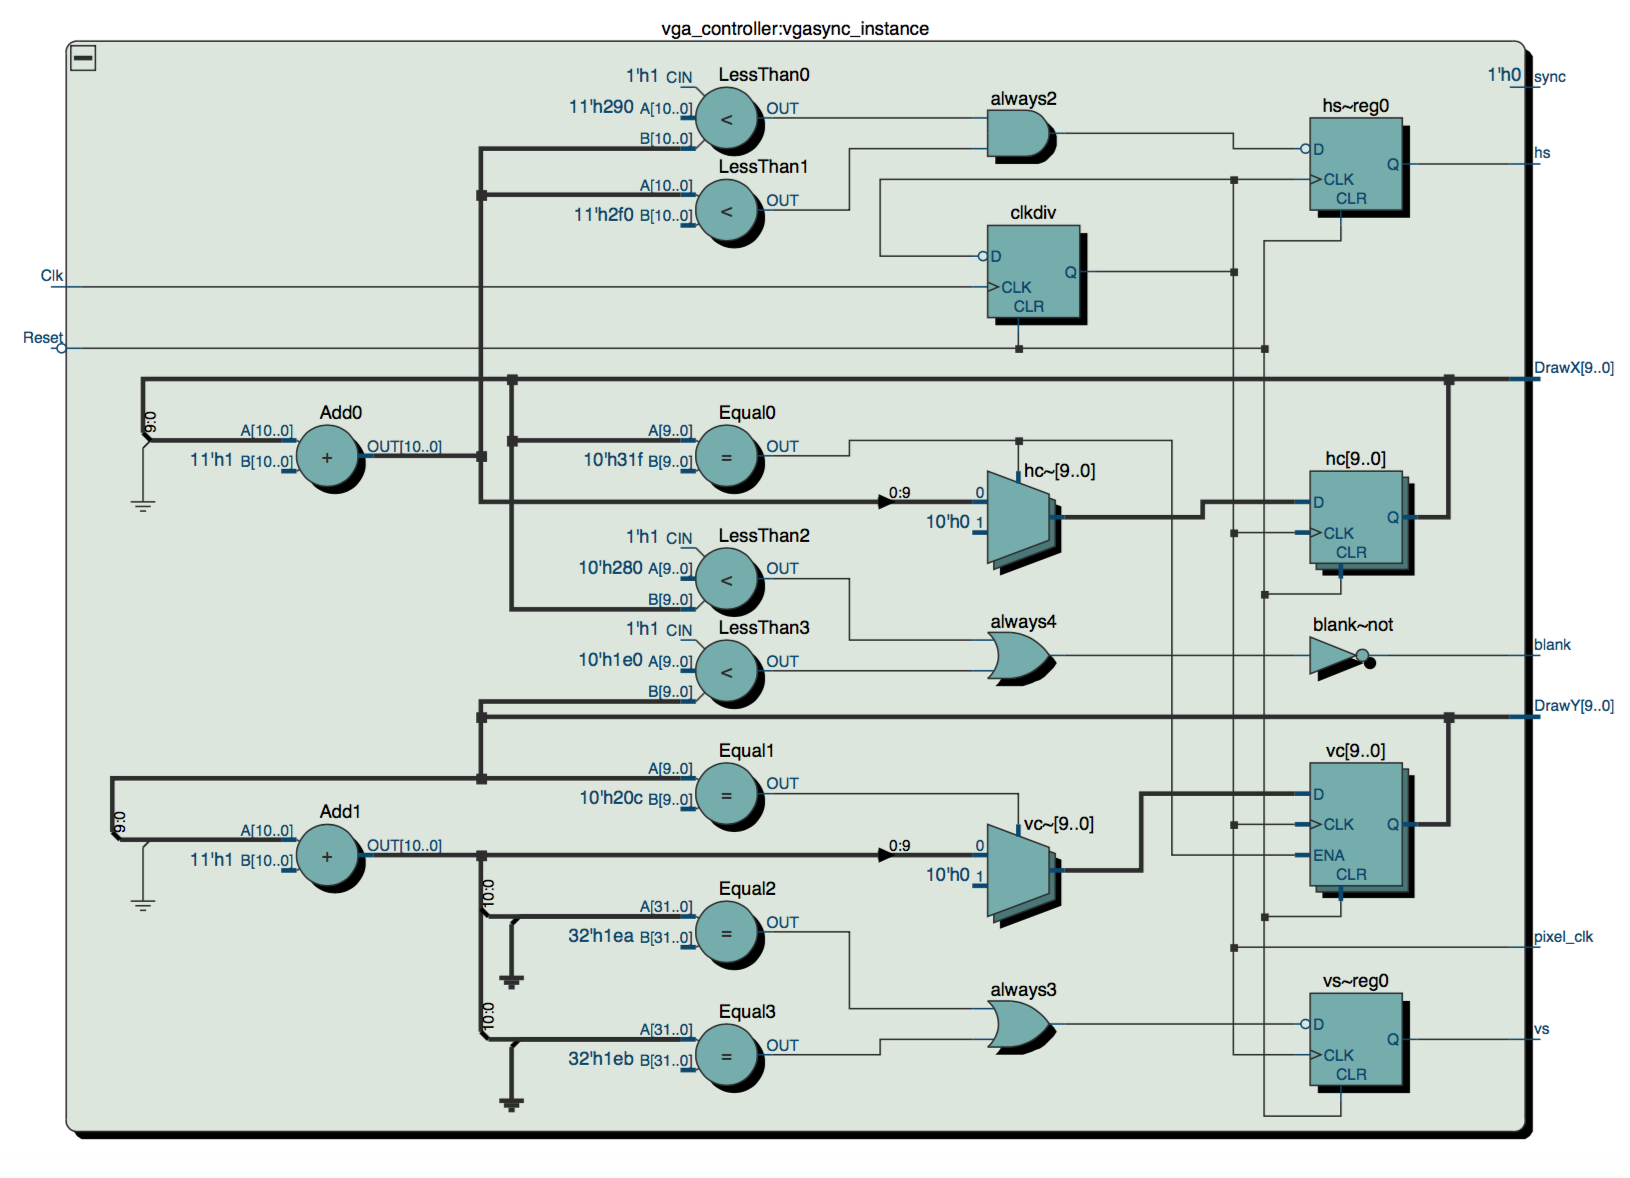
\includegraphics[scale=.5]{vga_diagram.png}
	\caption{VGA Circuit Diagram\label{fig:vga}}
\end{figure}

\begin{figure} [H]
	\centering
	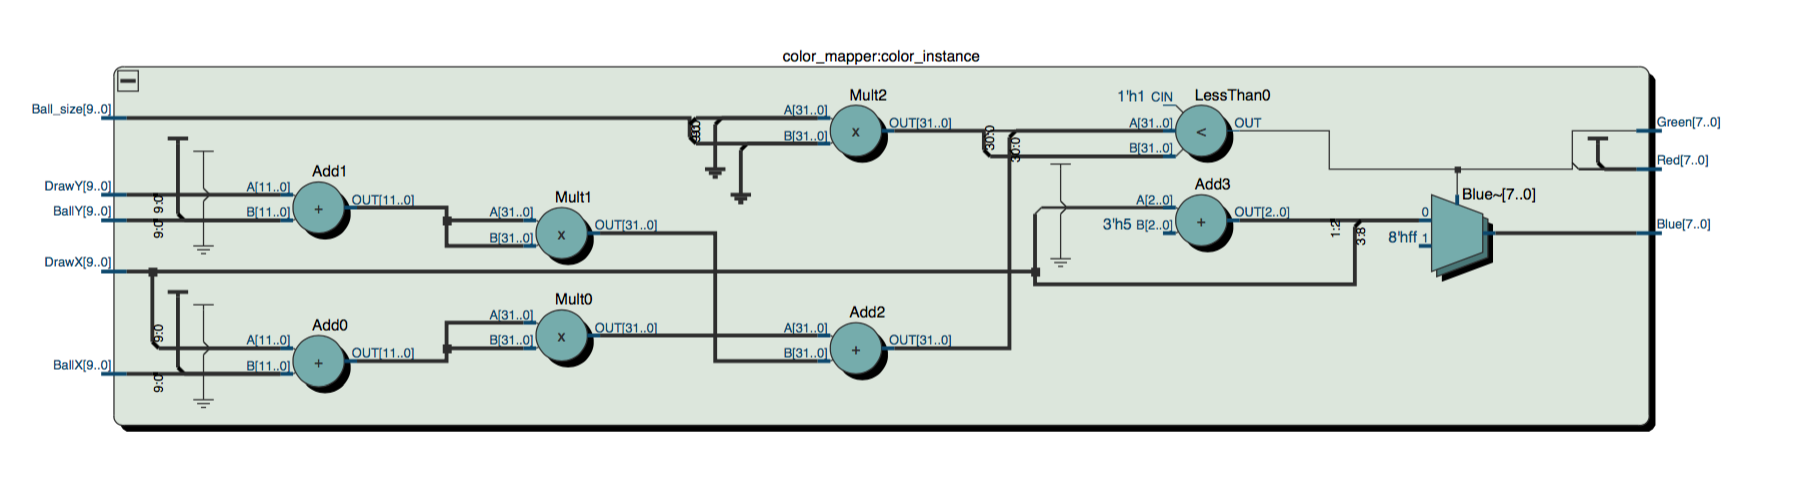
\includegraphics[scale=.5]{color_mapper_diagram.png}
	\caption{Color Mapper Circuit Diagram\label{fig:color_mapper}}
\end{figure}            

     

\section*{Appendix}


\end{document}
